\documentclass[border=10pt]{standalone}

\usepackage{tikz}
\usepackage{verbatim}
\usetikzlibrary{arrows.meta}
\usetikzlibrary{arrows,shapes,chains}

\tikzstyle{base} = [rectangle, rounded corners, draw=black, minimum width=1cm, minimum height=0.5cm, text centered, font=\sffamily]
\tikzstyle{activityStarts} = [base, fill=blue!30]
\tikzstyle{for} = [base,fill=blue!60]
\tikzstyle{startstop} = [base, fill=red!30]
\tikzstyle{activityjudge} = [base, rounded corners, draw=black,minimum width=4cm, minimum height=0.5cm, text centered, font=\sffamily,fill=green!30]
\tikzstyle{process} = [base, minimum width=2.5cm, fill=orange!15, font=\ttfamily]

\begin{document}

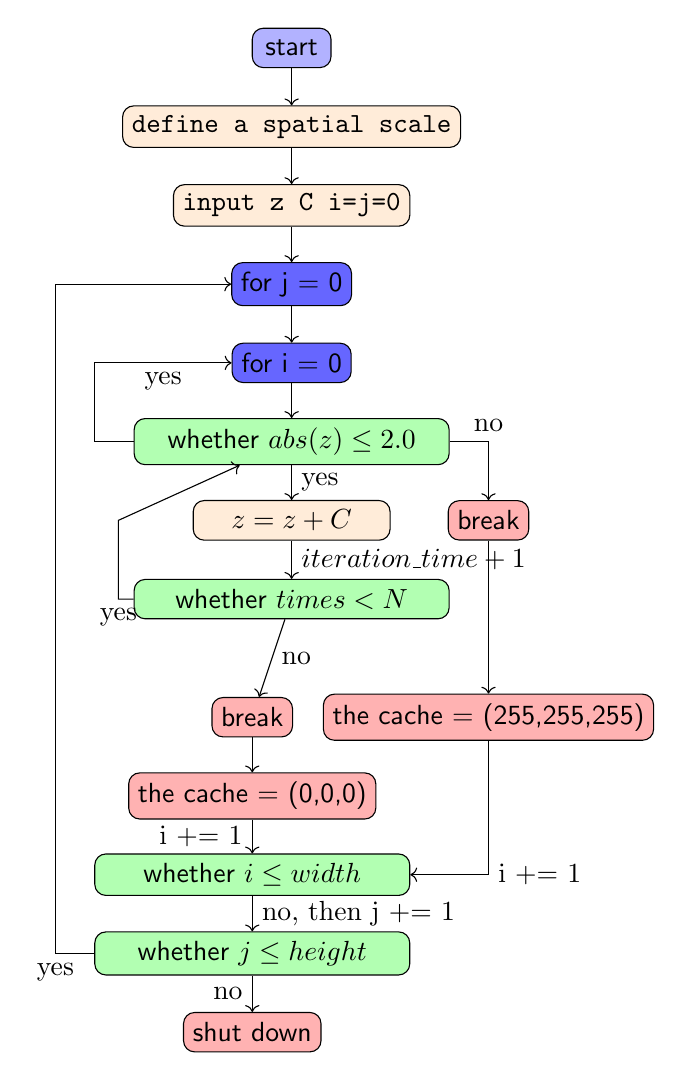
\begin{tikzpicture}[node distance=1cm]                                                   
    \node (start) [activityStarts]  {start};
    \node (define) [process, below of=start] {define a spatial scale};
    \node (input) [process, below of=define] {input z C i=j=0};
    \node (for1) [for, below of=input] {for j = 0};
    \node (for2) [for, below of=for1] {for i = 0};
    \node (if1) [activityjudge, below of=for2] {whether $abs(z) \le 2.0$};
    \node (Interation) [process, below of=if1] {$z = z + C$};
    \node (break1) [startstop, right of=Interation, xshift=1.5cm] {break};
    \node (output1) [startstop, below of=break1,yshift=-1.5cm] {the cache = (255,255,255)};
    \node (if2) [activityjudge, below of=Interation] {whether $times < N$};
    \node (break2) [startstop, left of=output1, xshift=-2cm] {break};
    \node (output2) [startstop, below of=break2] {the cache = (0,0,0)};
    \node (if3) [activityjudge, below of=output2] {whether $i \le width$};
    \node (if4) [activityjudge, below of=if3] {whether $j \le height$};
    \node (stop) [startstop, below of=if4] {shut down};

    \draw[->] (start) -- (define);
    \draw[->] (define) -- (input);
    \draw[->] (input) -- (for1);
    \draw[->] (for1) -- (for2);
    \draw[->] (for2) -- (if1);
    \draw[->] (if1) -- node[anchor=west] {yes} (Interation);
    \draw[->] (Interation) --node[anchor=west] {$iteration\_time+1$} (if2);
    \draw[->] (if2) -- node[anchor=west] {no} (break2);
    \draw[<-] (if1) -- (-2.2,-6) |- node[anchor=north] {yes} (if2);
    \draw[->] (break2) -- (output2);
    \draw[->] (if1) -| node[anchor=south] {no} (break1);
    \draw[->] (break1) -- (output1);
    \draw[->] (output2) -- node[anchor=east] {i += 1} (if3);
    \draw[->] (output1) |- node[anchor=west] {i += 1} (if3);
    \draw[<-] (for2) -- node[anchor=north] {yes} (-2.5,-4) |- (if1);
    \draw[->] (if3) -- node[anchor=west] {no, then j += 1} (if4);
    \draw[->] (if4) -- node[anchor=east] {no} (stop);
    \draw[<-] (for1) -- (-3,-3) |- node[anchor=north] {yes} (if4);
\end{tikzpicture}

\end{document}
